\documentclass[class=scrartcl, crop=false]{standalone}

\usepackage[sexy]{evan}
\usepackage{nicematrix}
\NiceMatrixOptions{transparent}
\usetikzlibrary{shapes.geometric, calc}

\title{Math 235 Notes --- 10-02}

\begin{document}

\section{10-02}


\begin{theorem}
  Any n-cycle is the product of $(n - 1)$ transpositions.
  \begin{proof}

    $$(a_1 \ a_2 \ \dots \ a_n) = (a_1 \ a_n)(a_1 \ a_{n - 1})\dots(a_1 \ a_3)(a_1 \ a_2)$$
    An alternative proof:
    $$(a_1 \ a_2 \ \dots \ a_n) = (a_1 \ a_2)(a_2 \ a_3)\dots(a_{n - 1} \ a_n)$$
  \end{proof}
\end{theorem}

\begin{definition}
  An element $\sigma \in S_n$ is:
  \begin{enumerate}
    \ii
    \ul{Even} if $\sigma$ is the product of an even number of transpositions
    \ii
    \ul{Odd} if $\sigma$ is the product of an odd number of transpositions.
  \end{enumerate}
  \begin{theorem}
    No $\sigma \in S_n$ is both even and odd.
    \begin{note}
      This means that any odd $\sigma$ can only be expressed as a product of an odd number of transpositions.
    \end{note}
    \begin{proof}
      Matricies over $\RR$ have det positive or negative. Positive determinent maintains orientation. Negative determinent inverses orientation. An even element can be likened to a matrix with a positive determinent, while an odd element can be likened to a matrix with a negative determinent.
    \end{proof}
  \end{theorem}
\end{definition}

\begin{example}
  $(2 \ 3 \ 5 \ 7 \ 9)$ is even because it is the product of four transpositions ($n - 1$).

  $(1 \ 8 \ 6 \ 2)$ is odd because it is the product of three transpositions ($n - 1$).
\end{example}

\begin{theorem}
  The set of even permutations of $S_n$ is a subgroup. $A_n \subset S_n$, \ul{alternating group}.
\end{theorem}
\begin{proof}
  Identity Element: $() = (1 \ 2)(1 \ 2)$ 

  Inverse: $() \in A_n$. Need to prove that $\sigma \in A_n \Rightarrow \sigma^{-1} \in A_n$.Indeed:
  $$\sigma = (a_1 \ b_1)(a_2 \ b_2)\dots(a_k \ b_k)$$
  $$\sigma = (a_k \ b_k)\dots(a_2 \ b_2)(a_1 \ b_1)$$

  Closure: $\sigma, \phi \in A_n \Rightarrow \sigma \cdot \phi \in A_n$. Even number of permutations times even number of permutations gives an even number of permuatations which is in $A_n$.
  \begin{note}
    $|A_n| = \frac{1}{2}|S_n|$.
  \end{note}
\end{proof}

Understanding $A_4 \subset S_4$.

Listing elements in $S_4$.
$S_4 = $
$$\{()\}$$
$$\{(1 \ 2)(3 \ 4), (1 \ 3)(2 \ 4), (1 \ 4)(2 \ 3)\}$$
\begin{gather*}\{
  (1 \ 2 \ 3), (1 \ 3 \ 2) \\
  (1 \ 2 \ 4), (1 \ 4 \ 2) \\
  (1 \ 3 \ 4), (1 \ 4 \ 3) \\
(2 \ 3 \ 4), (2 \ 4 \ 3) \}
\end{gather*}
\begin{note}
  $S_4$ "is"  an isometry group of tetrahedron.

  $A_4$ "is" the subgroup of its rigit motions.
\end{note}

\subsection{Cosets and Lagrange's Theorem}

Let $H \subset G$ be a subgroup.

Let $g \in G$.

The \ul{left coset} of H \ul{represented by g} is $gH = \{gh: h \in H\}$.

The \ul{right coset} of H \ul{represented by g} is $Hg = \{hg: h \in H\}$. 

Usually $gH \neq Hg$. (If equal just call them cosets if you'd like).

\begin{example}
  Misleading but simple example.

  $G = \ZZ_{12}, H = \langle 4 \rangle = \{0, 4, 8\}.$

  $$0 + H = 4 + H = 8 + H = \{0, 4, 8\}$$
  $$1 + H = 5 + H = 9 + H = \{1, 5, 9\}$$
  $$2 + H = 6 + H = 10 + H = \{2, 6, 10\}$$
  $$3 + H = 7 + H = 11 + H = \{3, 7, 11\}$$

  \begin{note}
    Notation can be confusing. $gh$ means binary operation between g and h so when binary operation is $+$ it means $g + h$.
  \end{note}

  Cosets formed a partition of the group.

  Review: What is a partition? Disjoint subsets that unionize to form a set.
\end{example}

\begin{example}
  $$H = \{1, -1, i, -i\} \subset \QQ_8$$
  $$1 \cdot H = \{1 * 1, 1 * -1, 1 * i, 1 * -i\}$$
  $$jH = \{j * 1, j * -1, j * i, j * -i\} = \{j, -j, -k, k\} = Hj$$
  \begin{note}
    These form a partition of the quaternions.
  \end{note}
\end{example}

\begin{example}
  $$K \subset \QQ_8$$
  $$K = \{1, -1\}$$
  \begin{gather*}
    1K = \{1, -1\} \\
    iK = \{i, -i\} \\
    jK = \{j, -j\} \\
    kK = \{k, -k\}
  \end{gather*}
  \begin{note}
    For all of these, a left coset is a right coset.
  \end{note}
\end{example}

\begin{example}
  $D_8$. Symmetries of a regular octogon. 
  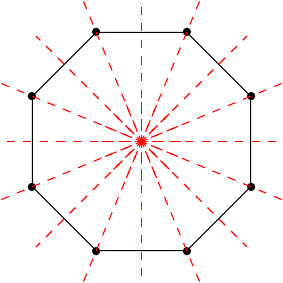
\begin{tikzpicture}[scale=3]
  \def\rps{8} % regular polygon sides
  \node (a) 
  [draw,  blue!0!black,rotate=90,minimum size=3cm,regular polygon, regular polygon sides=\rps] at (0, 0) {}; 

  \foreach \x in {1,2,...,\rps}
    \fill (a.corner \x) circle[radius=.5pt];
    \foreach \x in {1,2,...,\rps}{
    \draw [red,dashed, shorten <=-0.5cm,shorten >=-0.5cm](a.center) -- (a.side \x);
    \draw [red,dashed, shorten <=-0.5cm,shorten >=-0.5cm](a.center) -- (a.corner \x);}

  \end{tikzpicture}

  $$D_8 = \{r_i, \frac{i}{8}2\pi: 0 \leq i \leq 7\}$$
  Subgroup (Same as the isometry of a rectangle living inside): $$H = \{r_1, r_5, 0, \pi\}$$

  \begin{note}
    Product of rotation with rotation is a rotation. Product of a rotation with a reflection is a reflection. Product of a reflection with a reflection is a rotation.
  \end{note}

  \begin{gather*}
    0H = H \\
    \frac{\pi}{8}H = \{r_2, r_6, \frac{\pi}{8}, \frac{5\pi}{8}\} \\
    \frac{2\pi}{8}H = \{r_3, r_7, \frac{2\pi}{8}, \frac{6\pi}{8}\} \\
    \frac{3\pi}{8}H = \{r_4, r_0, \frac{3\pi}{8}, \frac{7\pi}{8}\} \\
    H\frac{\pi}{8} = \{r_0, r_4, \frac{\pi}{8}, \frac{5\pi}{8}\} 
  \end{gather*}
  \begin{note}
    Finding the product of a reflection and a rotation can be tricky. See how the composition affects a single point, and then identity a single rotation that affects the point in the same way.
  \end{note}
\end{example}

\begin{theorem}
  Lem 6.2. Let $g_1, g_2 \in G$ and $H \subset G$ be a group.

  TFAE (similar for right cosets)

  \begin{enumerate}
    \ii
    $g_1H = g_2H$ 
    \ii
    $Hg_1^{-1} = Hg_2^{-1}$. There is a bijection from a group to itself. Most obvious is identity bijection, but another one is every element to its inverse. In order to prove that statements 1 and 2 imply one another, use $\phi: G \to G, \phi(g) = g^{-1}. \phi$ is a bijection.$\phi(g_1h) = h^{-1}g_1^{-1} \Rightarrow \phi(gH) \subset Hg^{-1}$.
    \ii
    $g_1H \subset g_2H$ 
    \ii
    $g_2 \in g_1H$
    \ii
    $g_1^{-1}g \in H$. Reading this statement: "The difference between $g_1$ and $g_2$ lies in H.
  \end{enumerate}

  \begin{proof}
    $1 \Leftrightarrow 5$.

    $\Rightarrow$. Suppose $g_1^{-1}g_2 \in H$, then $g_2^{-1}g_1 = (g_1^{-1}g_2)^{-1} \in H$.

    Therefore $g_1H \subset g_2H$ because $g_1h = (g_2g_2^{-1})g_1h = g_2(g_2^{-1}g_1)h \in g_2H$. ($g_2h'$ with $h' \in H$).

    $\Leftarrow$. ( $g_1H = g_2H) \Rightarrow (g_1e \in g_2H) \Leftrightarrow (g_1 \in g_2H) \Rightarrow (g_1 = g_2h$ for some $h\in H) \Rightarrow g_2^{-1}g_1 = h \in H$.
  \end{proof}


\end{theorem}

\begin{theorem}
  Lem 6.4. Let $H \subset G$ be a subgroup. The left (or right) cosets of H form a partition of G.
  \begin{proof}
    Look:
    $$G = \bigcup_{g\in G}gH \ \text{because} \ g = ge \in gH$$
    If $g_1H\cap g_2H \neq \varnothing$, then $g_1H = g_2H$ because if $g_1h_1 = g_2h_2$, then $g_1^{-1}g_2 = h_1h_2^{-1} \in H$, hence $g_1H = g_2H$.
  \end{proof}
\end{theorem}

\begin{definition}
  Let $[G:H]$ be the \ul{index} of H in G denote the number of left cosets of H in G.
  \begin{example}
    $$[D_8:\{r_1, r_5, 0, \pi\}] = 4$$
    $$[\ZZ_{12}:\{0, 4, 8\}] = 4$$
    $$[\QQ_{8}:\{-1, 1\}] = 4$$
    $$[\QQ_{8}:\{-1, 1, i, -i\}] = 2$$
    $$[\ZZ: n\ZZ] = n$$
    $$[G:G] = 1$$
    $$[G:\{e\}] = |G|$$
  \end{example}
\end{definition}

\begin{theorem}
  6.4. Let $H \subset G$. The number of left cosets equals the number of right cosets.
  \begin{proof}
    The inversion map on $G$ sends left cosets to right cosets and right cosets to left cosets.

    Let L be the collection of left cosets and R be the collection of right cosets.

    Define bijection $\phi:L\to R$ by $\phi(gH) = Hg^{-1}$. Now to check that this function is well defined
    \begin{definition}.
      Well defined: independent of choice of representative.
    \end{definition}
    Check that if $gH = kH \Rightarrow \phi(gH) = \phi(kH)$.

    $$gH = kH \Rightarrow Hg^{-1} = Hk^{-1} \Rightarrow \phi(gH) = \phi(kH).$$

    Now check that $\phi$ is injective.

    $$ [\phi(gH) = \phi(kH)] \Rightarrow [Hg^{-1} = Hk^{-1}] \Rightarrow [gH = kH] $$

    Now check that $\phi$ is surjective.

    $Hx = H(x^{-1})^{-1} = \phi(x^{-1}H)$
  \end{proof}
\end{theorem}

\end{document}
